\documentclass[a4paper,10pt]{article}

% Kommentare: Alles hinter dem Zeichen "%" wird ignoriert.

% Zus"atzliche Pakete einbinden:
\usepackage[utf8]{inputenc} % So können Umlaute auch direkt eingegeben werden.
\usepackage{ngerman}  % Deutsche Sprachumgebung (neue Rechtschreibung)
\usepackage{amsmath}  % erweiterter Formelsatz
\usepackage{amssymb}  % weitere mathematische Symbole
\usepackage{amsfonts} % sch"one Fonts besonders f"ur Formeln
\usepackage{graphicx} % Bilder einbinden
\usepackage{hyperref} % Dokumentnavigation
\usepackage{booktabs} % für schönere Linien in Tabellen
%\usepackage{fullpage} % minimale Seitenr"ander, ist allerdings nicht immer verfügbar, 
% daher die alternative:
\usepackage[margin=1in,includefoot,footskip=30pt]{geometry}

\usepackage[load-configurations=abbreviations]
{siunitx}                                       % package for units. Use 
                                                % \si{\ampere} or 
                                                % \SI{0.3}{\angstrom}
% Keine Einr"uckung bei neuem Paragraphen 
\parindent 0pt

%% Definitionen f"ur das Titelblatt
\title{Musterprotokoll} 
\author{G. Quast}
\date{1. August 2019}



%% Hier f"angt das eigentliche Dokument  an
\begin{document}

\maketitle

%% Folgendes k"onnte man noch zus"atzlich einschalten
%\tableofcontents
%\listoffigures
%\listoftables
\begin{abstract}
  Eine kleine \LaTeX-Vorlage für das Musterprotokoll zu
 "`Computergestützte Datenauswertung"'. Beispielhaft wird
 auch gezeigt, wie von einem Analyse-Script erzeugte
 Grafiken und Tabellen eingebunden werden können.

 Eine wesentlich umfassendere 
\href{http://fachschaft.physik.kit.edu/drupal/content/latex-vorlagen}
     {Protokollvorlage für das Anfängerpraktikum}
  bietet die Fachschaft Physik.
\end{abstract} 



\section{Vorbereitungen} % ----------------------------------------------------
\label{chap:intro}  % mit ref{chap:intro} kann man von anderer Stelle hierher verweisen

Statt der Beschreibung der physikalischen Grundlagen, Messaufbaus,
der Daten und der Auswertung eines Praktikumsversuchs wird hier 
ganz kurz das Übersetzen eines \LaTeX{}-Dokuments erklärt.

Zur Verwendung dieser einfachen Vorlage können Sie 
Text, Grafiken, Tabellen und Formeln 
löschen und durch eigenes Material ersetzen.

  Eine wesentlich umfassendere
  \href{http://fachschaft.physik.kit.edu/drupal/content/latex-vorlagen}
  {Protokollvorlage für das Anfängerpraktikum} bietet die Fachschaft 
  Physik.


\subsection{\LaTeX{} "`Übersetzen"'}
Ist Ihr System korrekt eingerichtet, können Sie mit dem Befehl \\
\verb|pdflatex ProtokollVorlage|\\
aus der Datei \verb|ProtokollVorlage.tex|, die den \LaTeX{}-Quelltext
für diese Datei enthält, das zugehörige pdf-Dokument erzeugen. 

Mit dem Betriebssystem \verb|Linux| geht das sehr komfortabel 
mit dem Befehl \\
\verb|make|,\\
der die in der Datei \verb|Makefile| enthaltenen Befehle für
die Quelldateien abarbeitet, die neuer sind als die zu erzeugende
Ergebnisdatei. 

\subsection{Formeln erstellen}
Die ganz besondere Stärke von \LaTeX{} ist das Erstellen und
Setzen von Formeln. In die spezielle Mathematik-Umgebung 
gelangt man mit dem \verb|$|-Zeichen. Mit dem Text \\[0.5pc]
\verb|$\sum_{i=0}^{\infty} a_i x^i$|\\[0.5pc]
erhält als Ausgabe $\sum_{i=0}^{\infty} a_i x^i$, die in den
Text eingebettet ist. 

Umfangreichere Formeln, die dann nicht innerhalb des Textes, 
sondern mit viel Freiraum gesetzt werden sollen, 
schließt man  so ein: \verb|\[ <formel> \]|.

Man kann eine Formel auch in eine spezielle Umgebung einfügen,
die gleichzeitig für eine fortlaufende Nummerierung und damit 
Referenzierbarkeit sorgt:  
\begin{verbatim}
\begin{equation}  \label{equ:formel1}
\pi/4=\sum_{k=0}^\infty \frac{(-1)^k}{2k+1}
\end{equation} 
\end{verbatim}
So erhält man die Ausgabe
\begin{equation} \label{equ:formel1}
\pi/4=\sum_{k=0}^\infty \frac{(-1)^k}{2k+1}
\end{equation}
Diese Gleichung kann mit der Angabe \verb|\ref{equ:formel1}| im
Text referenziert werden:  s. Gleichung\ref{equ:formel1}.

Die Formel\ref{equ:formel2} im Anhang zeigt ein noch komplexeres
Beispiel.


\subsection{Bilder einfügen}
Das Paket "`graphicx"' erlaubt das einbinden von Bildern. Durch 
\verb!\usepackage{graphicx}! im Kopf dieses Dokuments wurde das Paket 
geladen. Damit können jetzt Bild-Dateien, wie sie bei der Datenauswertung
erstellt werden, mit dem Befehl
\begin{verbatim}
\includegraphics[width=BREITE]{BILDDATEI}
\end{verbatim}
in das Dokument aufgenommen werden.

Es empfiehlt sich, das Bild noch in eine sogenannte \verb|figure|-Umgebung 
einzuschließen.  Damit wird das Bild automatisch platziert und man kann mit 
dem Befehl \verb|\caption| auch eine Bildunterschrift angeben.  
Dieses Beispiel (Abb.\ref{fig:bild1}) wurde durch folgende Zeilen erzeugt:
\begin{verbatim}
\begin{figure}[htbp]
  \centering
  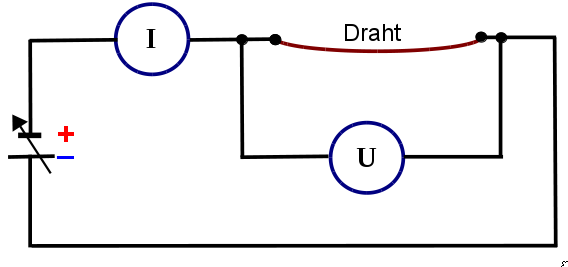
\includegraphics[width=0.5\linewidth]{Bild000}
  \caption{Beipiele f"ur eine eingebundene Bild-Datei.}
  \label{fig:bild1}
\end{figure}
\end{verbatim}
 
\begin{figure}[htbp]
  \centering
    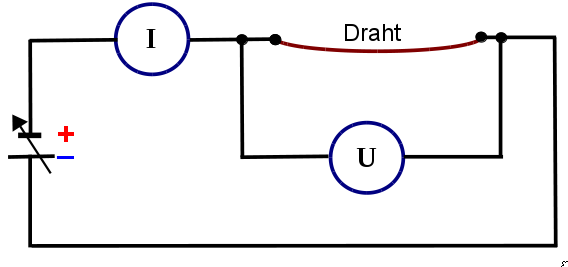
\includegraphics[width=0.5\linewidth]{Bild000}
    \caption{Beispiele für eine eingebundene Bild-Datei.}
    \label{fig:bild1}
\end{figure}

\subsection{Tabellen}
Tabellen einzubinden geht ganz analog: 
\begin{verbatim} 
\begin{table}[htbp]
  \centering
     \begin{tabular}{rr}
	\toprule
	$U ~/~  \si{V}$ & $I ~/~ \si{A}$\\
	\midrule
         1.0 & 0.5 \\
         1.5 & 0.7 \\
         2.0 & 1.1 \\
	\bottomrule
      \end{tabular}
    \caption{Beispiel einer eingebundenen Tabelle.}
    \label{tab:tabelle1}
\end{table}
\end{verbatim}

Mit diesem Text wurde die Tabelle \ref{tab:tabelle1} erzeugt.  
\begin{table}[htbp]
  \centering
     \begin{tabular}{rr}
	\toprule
	$U ~/~ (V)$ & $I ~/~ (A)$\\
	\midrule
         1.0 & 0.5 \\
         1.5 & 0.7 \\
         2.0 & 1.1 \\
	\bottomrule
      \end{tabular}
    \caption{Beispiel einer eingebundenen Tabelle.}
    \label{tab:tabelle1}
\end{table}

\newpage

\subsection{Automatisiertes Erzeugen und Einbinden von Tabellen und Grafiken aus \texttt{python}-Skript}

Es ist auch recht einfach möglich, Tabellen und Grafiken
in einem \verb|python|-Skript zu erstellen und mit Hilfe des
\verb|\include|-Befehls in ein Textdokument einzubinden.
Damit solche automatisiert erzeugten \texttt{include}-Dateien
gefunden werden, sollten sie in einem eigenen Verzeichnis,
z.\,B. \texttt{./analysis/} enthalten sein.
Die Tabelle\,\ref{tab:InputData} wurde mit Hilfe des Scripts
\verb|generate_ProtokollData.py| erzeugt, das eine Funktionsanpassung
an die in der Tabelle enthaltenen Rohdaten vornimmt. 
Erzeugt wurde die Tabelle inklusive der Unterschrift mit Hilfe der
Funktion \verb|writeTeXTable()| aus dem Paket \verb|PhyPraKit|
und mit dem folgenden \LaTeX-Quelltext in das Dokument eingebunden:

\begin{verbatim}
\begin{table}[htbp]
  \centering
  \begin{tabular}{cccc}
\hline
X & $\sigma_X$ & Y & $\sigma_Y$\\
\hline
%\\
1 & 0.2 & 2.017 & 0.2017\\
2 & 0.2 & 2.569 & 0.2569\\
3 & 0.2 & 3.491 & 0.3491\\
4 & 0.2 & 4.567 & 0.4567\\
5 & 0.2 & 4.974 & 0.4974\\
6 & 0.2 & 7.049 & 0.7049\\
7 & 0.2 & 9.305 & 0.9305\\
8 & 0.2 & 9.839 & 0.9839\\
9 & 0.2 & 11.25 & 1.125\\
10 & 0.2 & 12.84 & 1.284\\

\hline
\end{tabular}
\caption{ToyData; außer den in der Tabelle angegbenen Unsicherheiten gibt es noch eine gemeinsame Unsicherheit von 0.1 auf die Y-Werte und eine gemeinsame relative Unsicherheit von 5.0\% auf die X-Werte.}
%\\

  \label{tab:InputData}
\end{table}
\end{verbatim}

\begin{table}[htbp]
  \centering
  \begin{tabular}{cccc}
\hline
X & $\sigma_X$ & Y & $\sigma_Y$\\
\hline
%\\
1 & 0.2 & 2.017 & 0.2017\\
2 & 0.2 & 2.569 & 0.2569\\
3 & 0.2 & 3.491 & 0.3491\\
4 & 0.2 & 4.567 & 0.4567\\
5 & 0.2 & 4.974 & 0.4974\\
6 & 0.2 & 7.049 & 0.7049\\
7 & 0.2 & 9.305 & 0.9305\\
8 & 0.2 & 9.839 & 0.9839\\
9 & 0.2 & 11.25 & 1.125\\
10 & 0.2 & 12.84 & 1.284\\

\hline
\end{tabular}
\caption{ToyData; außer den in der Tabelle angegbenen Unsicherheiten gibt es noch eine gemeinsame Unsicherheit von 0.1 auf die Y-Werte und eine gemeinsame relative Unsicherheit von 5.0\% auf die X-Werte.}
%\\

  \label{tab:InputData}
\end{table}

Die Ergebnisgrafik\,\ref{fig:Result} wurde ebenfalls im oben beschriebenen
\texttt{python}-Skript erzeugt und wie folgt eingebunden:

\begin{verbatim}
\begin{figure}[htbp]
  \centering
    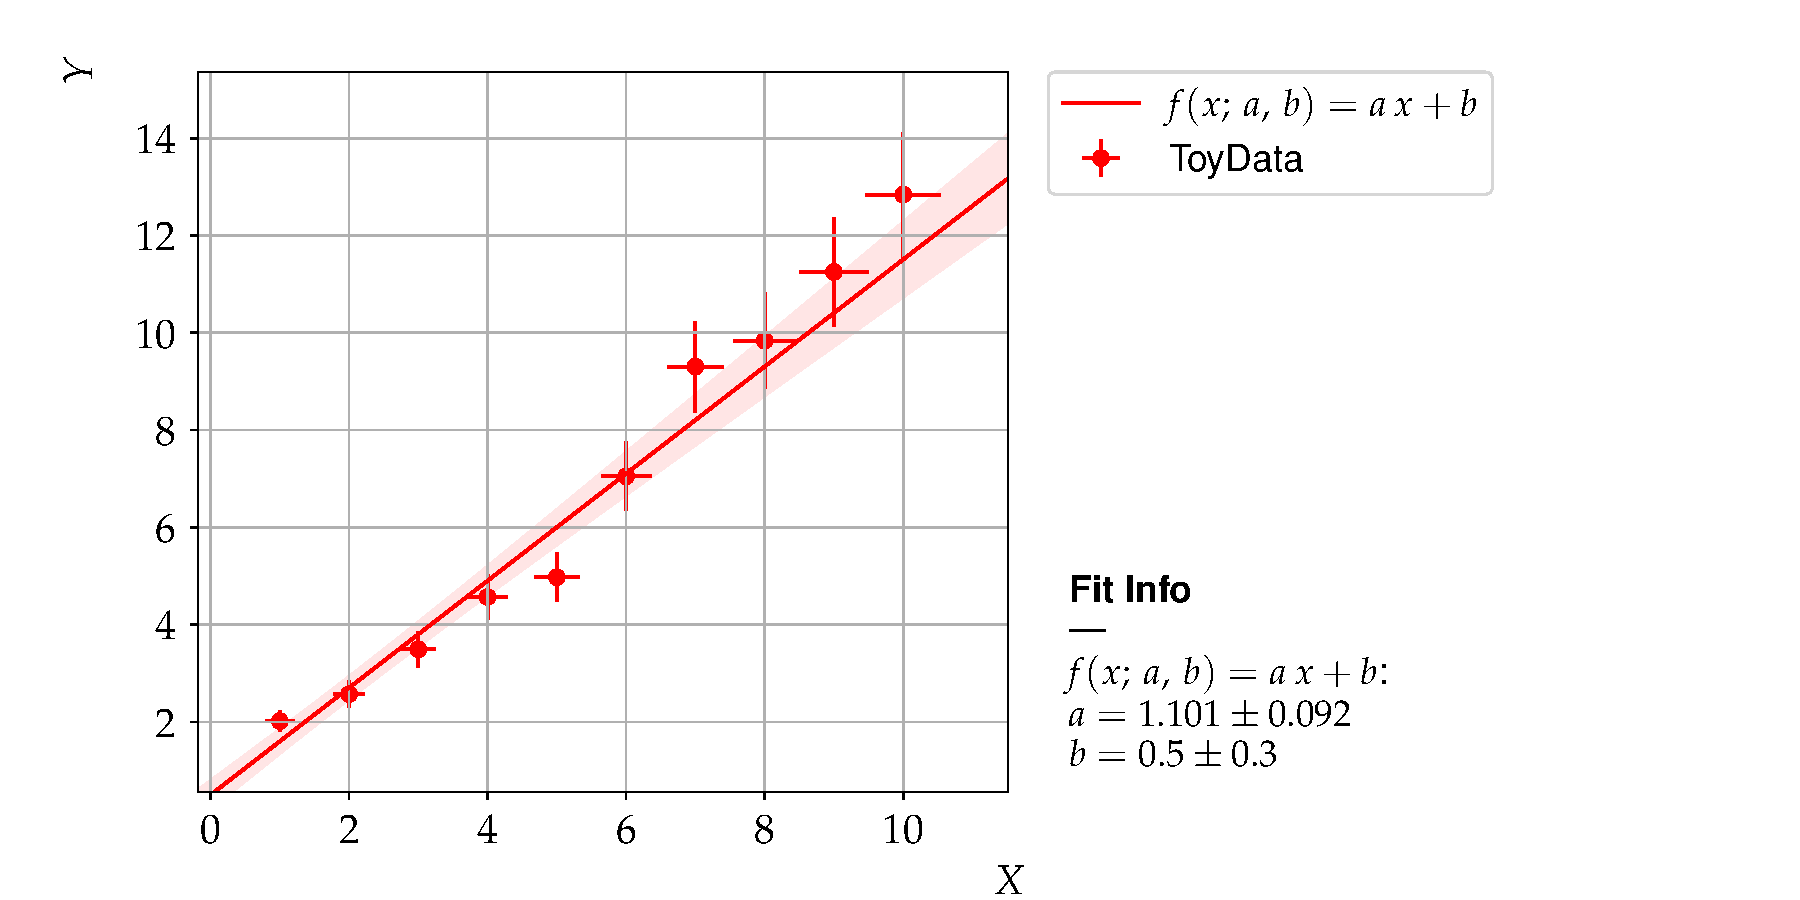
\includegraphics[width=1.0\linewidth]{analysis/Figure1}
    \caption{Grafik aus Skript generate\_ProtokollData.py.}
    \label{fig:Result}
\end{figure}
\end{verbatim}

\begin{figure}[htbp]
  \centering
    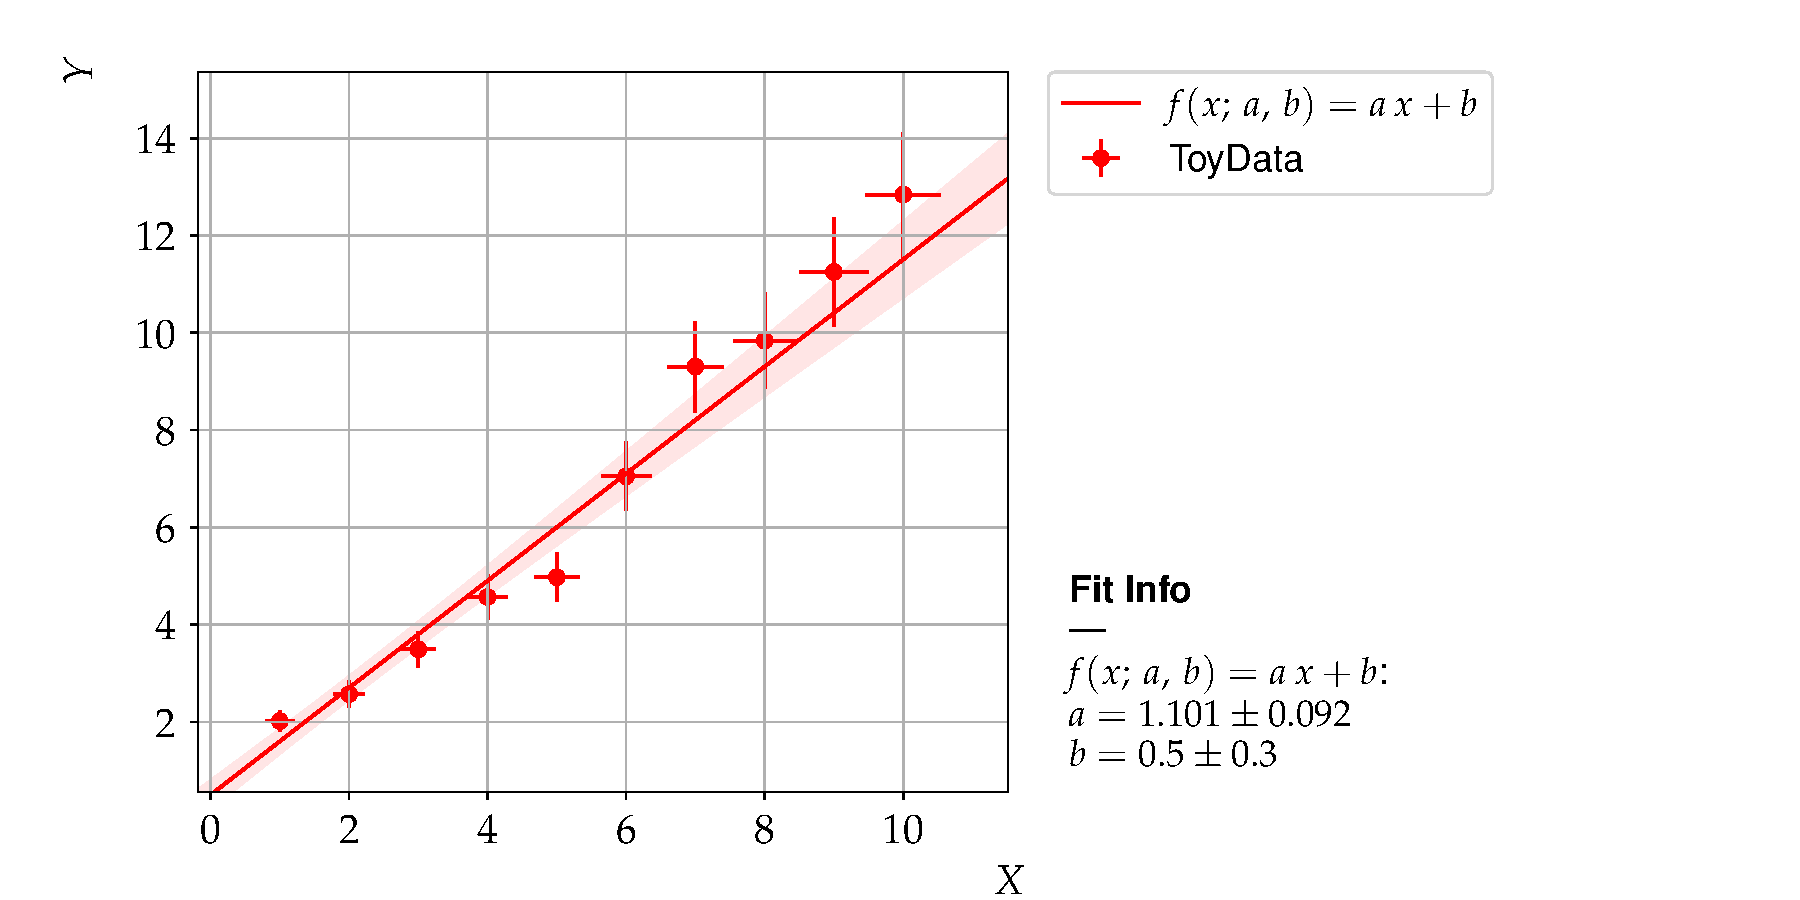
\includegraphics[width=0.8\linewidth]{analysis/Figure1}
    \caption{Grafik aus Skript generate\_ProtokollData.py.}
    \label{fig:Result}
\end{figure}

\pagebreak

\subsection{Literatur-Referenzen einfügen}
Für das Zitieren in \LaTeX{} ist der Befehl \verb|\cite[optionales]{key}| 
zuständig; \verb|key| ist dabei die Kurzbezeichnung in
der Literaturliste am Ende dieses Dokuments.
Hier als Beispiel die Referenz auf ein Buch zum 
Praktikum~\cite[S. 42]{EKS07}.


% appendix for more or less interesting calculations
\appendix % -------------------------------------------------------------

\section{Formelsammlung}

Formeln, verwendete Software-Werkzeuge und Methoden ...

\newcommand {\msum}{\displaystyle\sum}

\subsection{Lineare Regression}

Für die Anpassung einer Geraden $f(x)=p_1 + p_2 \, x$ 
an die Messungen $(x_i, y_i)$ mit den Unsicherheiten $\sigma_i$ 
erhält man mit den Abkürzungen
\begin{equation} \label{equ:formel2}
\begin{array}{lclcl}
S_{1~}  =~\msum_{i=1}^N \frac{1}{\sigma_i^2}\,,   &  &
S_{x~}  =~ \msum_{i=1}^N \frac{x_i}{\sigma_i^2}\,=\,\overline{x}\,S_1 \,,&  &
S_{y~}  =~ \msum_{i=1}^N \frac{y_i}{\sigma_i^2}\,=\,\overline{y}\,S_1 \,,\\[0.3pc]
S_{xx}  =~ \msum_{i=1}^N \frac{x_i^2}{\sigma_i^2}\,=\,\overline{x^2}\,S_1 \,,&  &
S_{xy}  =~ \msum_{i=1}^N \frac{x_i\,y_i}{\sigma_i^2}\,\,=\,\overline{xy}\,S_1 \,, & &
D_{~~}  =  {S_1S_{xx}-S_x^2} \\
\end{array}
\end{equation}
die Lösung
\[ \begin{array}{ccc c c c c }
\hat p_1&=&\frac{S_{xx}S_y-S_xS_{xy}}{D}\,, & & 
{\sigma_{p_1}}^2=\frac{S_{xx}}{D}\,, \\[0.3pc]
\hat p_2&=&\frac{S_1S_{xy}-S_xS_y}{D}\,,   & &
{\sigma_{p_2}}^2=\frac{S_{1}}{D}\,,        & & 
V_{12}=\frac{-S_{x}}{D}\,.           \\
\end{array}
\]


% THEBIBLIOGRAPHY
\begin{thebibliography}{000}
     \bibitem{EKS07} {Eichler, H. J. AND Kronfeldt, H.-D. AND Sahm, J.},
                     {Das Neue Physikalische Grundpraktikum}, {Springer DE},
                     {2016}.
\end{thebibliography}


\end{document}
